
\myChapter{Cammino minimo in un grafo}
In questo capitolo mostreremo il lavoro di un GA volto alla ricerca del cammino minimo in un grafo, a partire da un nodo v\ped{i} e terminante in un nodo v\ped{j}; l'implementazione dell'algoritmo \`e stata effettuata tramite l'uso del linguaggio Java. Nelle seguenti sezioni illustreremo il problema preso in considerazione e metteremo a confronto il GA con uno degli algoritmi pi\`u conosciuti.
\section{Descrizione del problema}
Il problema posto in esame in questo capitolo riguarda la ricerca del cammino minimo in un grafo orientato o non orientato (considereremo solo il secondo caso) da un vertice ad un altro, in modo pi\`u formale possiamo scrivere il tutto nella seguente maniera:
\vspace{3mm}

\textit{"Dato un grafo pesato (ossia un insieme di vertici V, un insieme di archi E ed una funzione f associante a ciascun arco un numero reale),  e dati due vertici distinti v\ped{i} e v\ped{j} $\in V$, trovare un cammino P=(e\ped{v\ped{i}v\ped{i+1}}, e\ped{v\ped{i+1}v\ped{i+2}}, e\ped{v\ped{i+2}v\ped{i+3}}, ..., e\ped{v\ped{j-1}v\ped{j}}) da v\ped{i} a v\ped{j} che minimizzi la somma $\sum_{e\in P} f(e)$."}
\vspace{3mm}

Sottolineamo che ogni vertice del cammino P deve essere adiacente a quello a lui precedente, ossia: preso un vertice v\ped{k} nel cammino P, fra lui e v\ped{k-1} deve esistere un arco che li connetta. Nel caso ogni arco avesse peso uguale ad 1, allora il cammino minimo risulterebbe essere quello contenente meno archi.
\vspace{3mm}

Il problema, cos\`i come lo abbiamo presentato, \`e noto anche come \textit{\textbf{problema del cammino minimo a singola coppia (single-pair shortest path problem)}}, in modo da distinguerlo dalle altre sue varianti (che non tratteremo nel corso delle successive sezioni):

\begin{itemize}
    \item \textbf{Problema del cammino minimo a singola fonte (single-source shortest path problem),} nel quale occorre trovare il cammino minimo da un singolo vertice verso tutti gli altri; sottolineiamo che ogni algoritmo risolvente tale problema, com'\`e evidente, \`e sicuramente in grado risolvere anche il single-pair shortest path problem (di fatto quest'ultimo lo rispecchia appieno, tranne nel criterio d'arresto);
    \item \textbf{Problema del cammino minimo a singola destinazione (single-destination shortest path problem),} consiste nel trovare il cammino minimo in un grafo diretto a partire da ogni vertice verso un'unica destinazione.
    \item \textbf{Problema del cammino minimo a coppie completo (all-pairs shortest path problem)}, versione amplificata di quello preso in esame in questo capitolo, infatti occorre trovare il cammino minimo fra tutte le coppie di vertici v\ped{i} e v\ped{j} nel grafo.
\end{itemize}

Dopo questa necessaria introduzione, nella prossima sezione presenteremo un algoritmo molto conosciuto, se non quello pi\`u usato ed analizzato in ambito scientifico, al fine di avere una migliore idea del problema stesso e della sua risoluzione.
\section{L'algoritmo di Dijkstra}
Una soluzione largamente apprezzata nelle ricerca del cammino minimo fu ideata da Edsger W. Dijkstra nel 1956 e pubblicata tre anni dopo, l'algoritmo ha innumerevoli varianti ma le sue forme pi\`u note riguardano il \textit{single-pair shortest path problem} (la prima in assoluto pensata da Dijkstra) ed il \textit{single-source shortest parth problem}. L'applicazione di tale algoritmo \`e vasta, in particolare \`e particolarmente apprezzata nei protocolli di routing, oltre ad essere usato come sub-routine in altri algoritmi di ricerca; ad oggi risulta essere, nella variante sviluppata da Fredman e Tarjan nel 1984, il miglior algoritmo nella risoluzione del problema che stiamo affrontando in questo capitolo.
\vspace{3mm}

L'idea dietro il funzionamento dell'algoritmo, che su parola di Dijkstra stesso fu concettualmente sviluppato in una ventina di minuti, scatur\`i dalla necessit\`a di trovare il percorso minimo per andare da una citt\`a ad un'altra; \`e immediatamente intuitivo considerare le citt\`a come vertici e le strade colleganti esse come gli archi di un grafo pesato in cui le distanze fra citt\`a corrispondono ai pesi degli archi, il tutto a patto di togliere ultieriori informazioni (semafori rossi, limiti di velocit\`a, segnali stradali ed ultieriori ostruzioni del percorso).

La facilit\`a con cui alcuni problemi si sposano con una trasformazione in un grafo, fa presto comprendere come questo approccio possa essere potente; senza ulteriori indugi illustreremo di seguito come l'algoritmo lavora.
\vspace{3mm}

Dato un vertice di partenza (noto anche come nodo inziale) in un grafo e data la \textit{distanzaY} la distanza che intercorre fra il nodo iniziale ed il nodo Y, l'algoritmo di Dijkstra assegner\`a alcuni valori iniziali di distanza e migliorer\`a in modo graduale di passo in passo la ricerca del cammino minimo:
\begin{enumerate}
    \item Impostare lo stato di tutti i nodi a "non visitato", creare al tempo stesso una lista che, di volta in volta, conterr\`a tali nodi ed un'altra lista per quelli gi\`a visitati. 
    \item Assegnare ad ogni nodo un valore di distanza iniziale, $0$ per il nodo di partenza ed un valore massimo per tutti gli altri ed inserire il nodo di partena nella lista dei "non visitati".
    \item Partendo dal nodo attuale (estratto dalla lista dei "non visitati"), calcolare la distanza \textit{provvissoria} fra tale nodo ed i suoi vicini non ancora visitati; successivamente, se la distanza \`e minore del valore assegnato al nodo su cui ci stiamo dirigendo, allora tale valore deve essere aggiornato, altrimenti non viene effettuato alcun cambio.
    \item Una volta che abbiamo terminato di considerare tutti i nodi vicini, inseriamo il nodo attuale nella lista dei "visitati".
    \item Se il nodo destinazione fosse gi\`a stato visitato, terminiamo l'esecuzione, altrimenti l'algoritmo continua fino ad aver visitato tutti i nodi (quest'ultimo approccio consente di calcolare il cammino minimo verso ogni vertice del grafo a partire dal quello designato come sorgente).
\end{enumerate}

Terminata questa doverosa premessa e spiegazione, mostriamo di seguito il codice Java relativo al funzionamento dell'algoritmo.
\definecolor{pblue}{rgb}{0.13,0.13,1}
\definecolor{pgreen}{rgb}{0,0.5,0}
\definecolor{pred}{rgb}{0.9,0,0}
\definecolor{pgrey}{rgb}{0.46,0.45,0.48}
%\usepackage{listings}
\lstdefinestyle{Java}{language=Java,
  showspaces=false,
  showtabs=false,
  numbers=left,
  frame=single,
  breaklines=true,
  showstringspaces=false,
  breakatwhitespace=true,
  commentstyle=\color{pgreen},
  keywordstyle=\color{pblue},
  stringstyle=\color{pred},
  basicstyle=\ttfamily,
  moredelim=[il][\textcolor{pgrey}]{$129$},
  moredelim=[is][\textcolor{pgrey}]{\%\%}{\%\%}
}
\begin{lstlisting}[style=Java]
public Iterator<Node> DijkstraAlgorithm(Node source, Node destination) throws Exception{
	if (!nodes.contains(source) || !nodes.contains(destination)) throw new Exception("Il nodo definito come iniziale o finale non appartiene al grafo");
		
	//Passo 1 e 2
	source.setDistance(0);
	ArrayList<Node> vNodes=new ArrayList<>();
	ArrayList<Node> nvNodes=new ArrayList<>();
	nvNodes.add(source);
		
	while (nvNodes.size()!=0) {
		Node n=minDistanceNode(nvNodes);
		nvNodes.remove(n);
		
		//siamo giunti a destinazione terminiamo, Passo 5
		if (n.equals(destination)) break;
		
		HashMap<Node, Integer> map=n.getConnectedNodes();
			
		//Passo 3
		for (Entry<Node,Integer> e: map.entrySet()) {
			Node m=e.getKey();
			
			 //necessaria per grafi non orientati
			if (vNodes.contains(m)) continue;
			
			int d=e.getValue().intValue();
			setDistance(m, n, d);
			nvNodes.add(m);
		}
			
		//Passo 4
		vNodes.add(n);
	}
	return destination.getPath();
}
\end{lstlisting}
\vspace{3mm}

Essendo l'algoritmo estremamente noto, abbiamo preso ispirazione da sue varie implementazioni circolanti nel web, in particolare la nostra versione (grazie al controllo a riga 24) permette l'uso sia per grafi orientati che non; i commenti presenti sono autoesplicativi se collegati ai 5 punti elencati prima, sottilineamo solamente i metodi \textit{minDistanceNode} e \textit{setDistance}.

Il primo permette la ricerca del nodo a minima distanza fra quelli non visitati, nel caso esso corrispondesse alla destinazione desiderata terminiamo il ciclo while (tolto questo controllo il metodo calcoler\`a i cammini minimi verso ogni nodo a partire da quello iniziale); il metodo setDistance imposta la distanza dal nodo attuale, estratto dalla lista dei "non visitati", verso un nodo ad esso connesso, nel caso la somma della distanza cumulativa del nodo attuale con il peso dell'arco collegante i due nodi sia minore della distanza cumulativa del nodo su cui vogliamo arrivare, allora aggiorneremo quest'ultimo valore ed i percorsi minimi provvisori.

Per avere una maggiore visione del codice, vi invitiamo a dare uno sguardo all'appendice a fine tesi, nella quale troverete ogni singolo sorgente usato nel corso dei vari capitoli.
%\vspace{3mm}
\section{Implementazione del GA}
Procediamo, finalmente, con l'illustrazione del codice del GA con annessa spiegazione delle varie scelte prese in sede di sviluppo del sorgente; per prima cosa, desideriamo sottolineare che l'algoritmo di Dijkstra ed il nostro algoritmo genetico appartengono alla stessa classe, ma le operazioni del GA sono definite nella classe \textit{Population.java}.

Il codice da noi sviluppato prende alcune delle idee viste in \cite{path3}, seppure apportando modifiche alle varie operazioni o eliminando quelle che abbiamo ritenuto eccessive.
\vspace{3mm}

Di seguito mostriamo la costruzione della popolazione iniziale su cui poi il GA eseguir\`a il proprio lavoro oltre alla chiamata del metodo che gestisce le sue operazioni di selezione, crossover e mutazione.
\begin{lstlisting}[style=Java]
public Chromosome ShortestPathGA(Node source, Node destination, int pSize, int maxGen, double pCrossover, double pMutation) throws Exception{
	if (nodes.size()==0) throw new Exception("Non sono stati inseriti nodi nel grafo");
	
	//Creo la popolazione e costruisco la matrice di adiacenza
	population=new Population(nodes.size(), pSize, this);
	population.buildMatrixDist(nodes.iterator());
	
	int j=0;
	while (j<pSize) {
		//Creo un cromosoma assegnandoli un percorso (geni) casuale fra sorgente e destinazione
		Chromosome c=new Chromosome(createRandomPath(source, destination));
		Iterator<Chromosome> itC=population.getChromosomes();
		
		//Controllo se tale percorso esiste gi\`a
		boolean hasSamePath=false;
		while (itC.hasNext()) {
			if (itC.next().hasSamePath(c)) {
				hasSamePath=true;
				break;
			}
		}
		if (!hasSamePath) {
			//Nel caso il cromosoma fosse unico (percorso differente dagli altri), lo aggiungo alla popolazione
			population.addChromosome(c);
			j++;
		}
	}
	
	//Eseguo il GA per un numero massimo di generazioni
	for (int i=0;i<maxGen; i++) {
		population.pathGA(pCrossover, pMutation);
	}
	return population.getFittest(); //Restituzione del miglior cromosoma
}
\end{lstlisting}
Dopo un primo controllo, il metodo provvede a creare la popolazione ed a costruire la matrice di adiacenza relativa ai nodi del grafo (tale matrice \`e usata solamente per il GA, l'algoritmo di Dijkstra non ne fa uso), successivamente costruisce cromosomi assegnando loro un percorso casuale da nodo iniziale a finale (l'idea approssima quanto espresso in \cite{path3}: un cromosoma viene aggiunto alla popolazione se e solo se il loro percorso (ovvero una sequenza di nodi corrispondente ai loro geni) risulta differente da tutti quelli gi\`a presenti nella popolazione. Questo \`e estremamente vitale per avere pi\`u diversit\`a nella popolazione, in modo da diminuire la possibilit\`a che l'algoritmo entri in stallo su soluzioni buone, ma non ottime, nelle sue prime iterazioni.

Dopo l'inizializzazione della popolazione, viene eseguito il metodo \textbf{pathGA} appartenente alla classe \textit{population} per \textit{maxGen} generazioni (numero scelto arbirtrariemente dal programmatore); il metodo termina restituendo il miglior cromosoma della popolazione finale.
\vspace{3mm}

Il metodo \textbf{pathGA} fa entrare il flusso del programma nel suo "nucleo", in quanto ha il compito di creare la nuova generazione di cromosomi a partire da quella precedente tramite i tre operatori che conosciamo gi\`a.
\begin{lstlisting}[style=Java]
public void pathGA(double pCrossover, double pMutation) {
	ArrayList<Chromosome> newGeneration=new ArrayList<>();
	while (newGeneration.size()<pSize) {
		//Selezione
		ArrayList<Chromosome> parents=selection();
		
		//Generazione di un numero casuale fra 0 ed 1
		Random r=new Random();
		double rDouble=r.nextDouble();
		
		//Crossover
		if (rDouble<pCrossover) {
			nCrossover++;
			ArrayList<ArrayList<Node>> sons=crossover(parents);
			
			//Mutazione
			mutation(sons, pMutation);
			
			//Aggiunta dei nuovi cromosomi alla popolazione
			newGeneration.add(new Chromosome(sons.get(0).iterator()));
			newGeneration.add(new Chromosome(sons.get(1).iterator()));
			
		}
	}
	newGeneration.forEach(c -> setFitness(c));
	Collections.sort(newGeneration, Chromosome.fitnessComparator);
	int i=newGeneration.size()-1;
	while (newGeneration.size()>pSize) {
		newGeneration.remove(i);
		i--;
	}
	chromosomes=newGeneration;
	best=chromosomes.get(0);
	bestFitness=best.getFitness();
}
\end{lstlisting}
Il metodo precedente rispecchia pienamente quanto detto nei capitoli passati riguardo al flusso d'esecuzione di un GA: viene creata la nuova generazione ed in seguito, fino a quando non viene raggiunta o superata la dimensione dell'attuale popolazione, vengono eseguite ripetute chiamate al metodo \textbf{selection}, il quale restituisce i due candidati genitori.

Viene, a questo punto, generato casualmente un numero reale: se esso risultasse minore del tasso di crossover, procederemo con la chiamata al metodo che si occupa di tale operazione. Dopodich\'e viene chiamato il metodo riguardante la mutazione con la successiva aggiunta dei due nuovi cromosomi alla popolazione.
%\vspace{3mm}

Al termine del ciclo principale, calcoliamo il valore di fitness (scelto come la somma delle distanze fra ogni nodo del percorso) per ogni cromosoma della nuova generazione, dopo di ci\`o riduciamo il numero di membri se necessario (potrebbe capitare con \textit{pSize} dispari di avere una generazione con dimensione maggiore di quella attuale) ed aggiorniamo i cromosomi della popolazione, calcolando al tempo stesso il migliore fra essi e la miglior fitness trovata.
\vspace{3mm}

Continuiamo l'analisi del codice sorgente con i tre metodi che implementano i tre operatori fondamentali, sui quali abbiamo gi\`a fatto abbastanza riflessioni nei capitoli precedenti: ci limiteremo ad illustrare i punti su cui differiscono da quanto visto nel capitolo 3.

Senza ulteriori premesse, presentiamo adesso il metodo relativo all'operatore di selezione.
\begin{lstlisting}[style=Java]
private ArrayList<Chromosome> selection() {
	//Dimensione del torneo
	int tSize=5;
	
	//Lista temporanea dei cromosomi
	ArrayList<Chromosome> tChroms=new ArrayList<>();
	
	chromosomes.forEach(c -> tChroms.add(c));
	Random r=new Random();
	
	//Cromosomi genitori
	ArrayList<Chromosome> parents=new ArrayList<>();
	
	while (parents.size()<2) {
		//Cromosomi partecipanti al torneo
		ArrayList<Chromosome> selChroms=new ArrayList<>();
		while (selChroms.size()<tSize) {
			int rInt=r.nextInt(tChroms.size());
			Chromosome c=tChroms.get(rInt);
			if (!selChroms.contains(c)) {
				selChroms.add(c);
			}
		}
		
		Collections.sort(selChroms, Chromosome.fitnessComparator);
		
		//Scelta del vincitore del torneo
		double p=0.75;
		double[] partialSums=new double[tSize];
		double sumP=0;
		for (int i=0;i<tSize;i++) {
			sumP+=p*Math.pow((1-p), i);
			partialSums[i]=sumP;
		}
		double rDouble=r.nextDouble()*sumP;
		int i=0;
		while (partialSums[i]<rDouble) {
			i++;
		}
		parents.add(selChroms.get(i));
		tChroms.remove(i);
	}
	return parents;
}
\end{lstlisting}
La selezione avviene nella sua variante a torneo con dimensione uguale a 5 e la scelta del miglior partecipante al torneo avviene con una probabilit\`a pari a $0.75$; successivamente il vincitore viene estratto dalla lista temporanea dei cromosomi, affinch\'e non possa essere scelto una seconda volta. Il metodo restituisce una lista contenente i due possibili genitori, i quali parteciperanno al crossover con probabilit\`a \textit{pCrossover}.
\vspace{3mm}

Parlando di crossover, \`e doveroso sottolineare che i cromosomi, come si potrebbe aver intuito, possono avere dimensioni differenti: questo causa un piccolo problema in questa fase, in quanto diventa necessario (ai fini della generazione del crossover point) calcolare la minima dimensione fra i due genitori per non incorrere in eccezioni.
\begin{lstlisting}[style=Java]
private ArrayList<ArrayList<Node>> crossover(ArrayList<Chromosome> parents) {
	//Estrazione dei due genitori dalla lista
	Chromosome parent1=parents.get(0);
	Chromosome parent2=parents.get(1);
	
	ArrayList<Node> son1=new ArrayList<>();
	ArrayList<Node> son2=new ArrayList<>();
	
	//Ottenimento dei geni dei due genitori
	Iterator<Node> itP1=parent1.getGenes();
	Iterator<Node> itP2=parent2.getGenes();
	
	//Calcolo della dimensione minima
	int minSize=parent1.getSize();
	if (parent2.getSize()<minSize) minSize=parent2.getSize();
	
	//Generazione del punto di crossover
	Random r=new Random();
	int rIndex=r.nextInt(minSize-1);
	
	//Crossover a punto singolo
	int i=0;
	while (i<rIndex) {
		son1.add(itP1.next());
		son2.add(itP2.next());
		i++;
	}
	while (itP1.hasNext()) {
		son2.add(itP1.next());
	}
	while (itP2.hasNext()) {
		son1.add(itP2.next());
	}
	
	//Restituzione dei due figli
	ArrayList<ArrayList<Node>> sons=new ArrayList<>();
	sons.add(son1);
	sons.add(son2);
	return sons;
}
\end{lstlisting}
A differenza di quanto fatto da \cite{path3} (in cui il crossover point viene scelto fra geni identici dei due cromosomi), generiamo il punto di crossover \textit{rIndex} nell'intervallo [0, minSize-1], i tre while eseguono lo stesso lavoro di un crossover a punto singolo che abbiamo potuto osservare nel capitolo 3; il metodo termina restituendo una lista di percorsi e non i due cromosomi: questa soluzione \`e scelta in modo che la mutazione avvenga prima dell'effettiva creazione dei due oggetti relativi ai figli, modificare direttamente un array \`e molto pi\`u semplice che lavorare con iteratori per poi aggiornare i geni dell'individuo.
\vspace{3mm}

Terminiamo la sezione con il metodo riguardante la mutazione, niente di nuovo rispetto a quanto visto nei capitoli precedenti se non per una modifica che risulta fondamentale per la riuscita dell'algoritmo in s\'e.
\begin{lstlisting}[style=Java]
private void mutation(ArrayList<ArrayList<Node>> individuals, double pMutation) {
	Random r=new Random();
	for (int i=0;i<individuals.size();i++) {
		ArrayList<Node> son=individuals.get(i);
		for (int j=0;j<son.size()-1;j++) {
			double rDouble=r.nextDouble();
			
			//Se la mutazione avviene, trovo un nuovo percorso dal nodo scelto verso la destinazione
			if (rDouble<pMutation) {
				nMutation++;
				Node n=son.get(j);
				Node d=son.get(son.size()-1);
				Iterator<Node> itN= graph.createRandomPath(n, d);
				
				//Eliminimo gli elementi successivi al nodo che ha subito la mutazione
				for (int k=son.size()-1;k>=j;k--) {
					son.remove(k);
				}
				
				//Aggiungo il percorso
				while (itN.hasNext()) son.add(itN.next());
				break;
			}
		}
		
		//Elimino i nodi dupilcati
		son=(ArrayList<Node>)son.stream().distinct(). collect(Collectors.toList());
	}
}
\end{lstlisting}
La mutazione, che agisce unicamente su un gene, crea un percorso casuale (con lo stesso metodo \textbf{createRandomPath} dell classe Graph) a partire dal gene stesso fino alla destinazione; in seguito elimina i geni successivi a quello da cui abbiamo calcolato il percorso ed aggiorna quello totale, eliminando inoltre i potenziali geni duplicati creatisi con il crossover e/o con la mutazione.
\vspace{3mm}

L'algoritmo, come si pu\`o notare dai codici esaminati, fa uso di altri metodi di supporto non inseriti in questa sezione: come sempre, saranno disponibili al termine della tesi nell'apposita appendice. L'obiettivo che rimane adesso \`e mostrare l'efficacia effettiva del nostro approccio.
\section{Analisi di un esempio}
In questa sezione porremo sotto esame il comportamento del nostro GA appena descritto, ma prima occorre senza dubbio avere a disposizione un grafo su cui operare. Grazie ad un tool online trovato su graphonline.ru e alla costruzione degli oggetti relativi ai nodi ed agli archi in Java, siamo riusciti a creare un grafo non orientato con $20$ vertici numerati da $0$ a $19$, dopodich\'e abbiamo inserito i dati nel nostro programma (nodo iniziale e nodo finale) ed abbiamo applicato l'algoritmo di Dijkstra.
\begin{figure}[H]
    \centering
    \hfill
    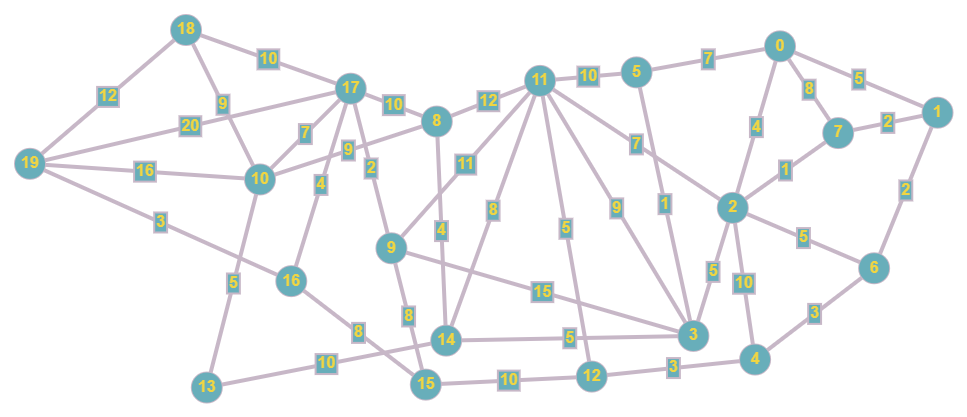
\includegraphics[width=1\textwidth]{Images/graph.png}
    \hspace*{\fill}
    \caption{Il grafo preso in esame}
    \label{fig:graph}
\end{figure}
Il nostro obiettivo consisteva nel trovare in tale grafo il cammino minimo da un nodo iniziale ad uno finale: per tutta la sezione supporremo di dover partire dal nodo $0$ e terminare nel nodo $19$; tale cammino sar\`a vitale nell'analisi del funzionamento del GA.
\vspace{3mm}

Per testare il funziomento dell'algoritmo di Dijkstra da noi implementato lo abbiamo messo a confronto con un calcolatore online: i risultati sono stati tutti positivi, dunque per testare il lavoro del nostro GA ci siamo basati sulle risposte dell'algoritmo di Dijkstra costruito nella nostra classe Graph.

Come detto poco fa, il nostro scopo era calcolare il minimo cammino dal nodo $0$ al nodo $19$, nell'immagine sottostante si pu\`o osservare da quali nodi sia formato.
\begin{figure}[H]
    \centering
    \hfill
    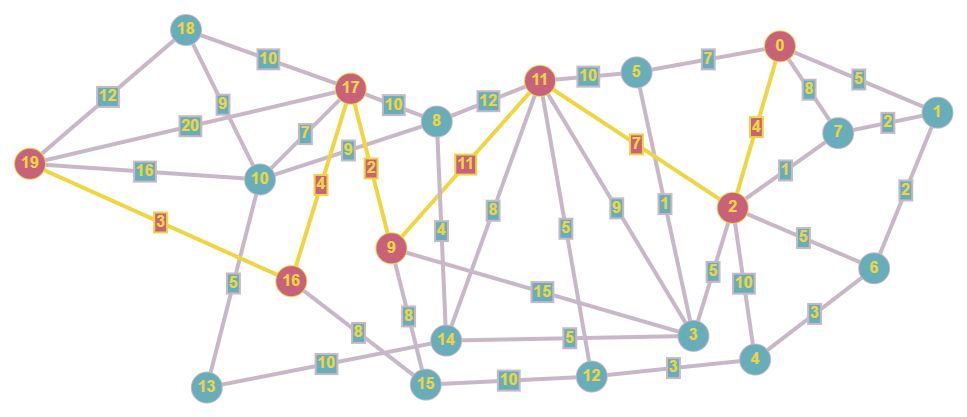
\includegraphics[width=1\textwidth]{Images/path.png}
    \hspace*{\fill}
    \caption{Il cammino minimo calcolato dall'algoritmo di Dijkstra}
    \label{fig:path}
\end{figure}
Il cammino risulta avere una lunghezza pari a 31, questo ci permette di avere un valore di riferimento utile per mostrare ed analizzare i risultati scaturiti dal lavoro del GA.
\vspace{3mm}

L'algoritmo genetico ha dato risultati molto eterogenei fra di loro a seconda dei parametri inseriti, in ogni caso precisiamo che i nosti valori di partenza corrispondono a:
\begin{itemize}
    \item Numero massimo di iterazioni (\textit{maxIt}), $30$;
    \item Dimensione della popolazione (\textit{pSize}), $40$;
    \item Tasso di mutazione, $0.1$;
    \item Tasso di crossover, $0.90$
    \item Dimensione del torneo (\textit{tSize}), $5$;
    \item Tasso di scelta del migliore del torneo, $0.75$;
\end{itemize}
%aver mai alterato il numero massimo di iterazioni ($30$), la dimensione del torneo di selezione ($5$) e la relativa probabilit\`a di scelta del vincitore ($0.75$).
Nella nostra analisi abbiamo agito sui primi cinque parametri, ma non abbiamo rilevato enormi differenze agendo sui tassi di mutazione e crossover (i migliori risultati sono stati ottenuti con i valori specificati e che rimarrano gli stessi per tutta l'analisi), di conseguenza sono stati la dimensione della popolazione  e del torneo uniti al numero massimo di iterazioni ad aver determinato maggiormente l'efficacia del nostro algoritmo.
%abbiamo agito sulla dimensione della popolazione, sulla dimensione del torneo di selezione, sul numero massimmo di iterazioni, sul crossover e sulla mutazione; ma sono state sicuramente le prime $3$ ad aver avuto il maggior impatto rispetto alle altre due.
\vspace{3mm}

Per ogni valore di \textit{pSize} (dimensione della popolazione, lasciando immutati tutti gli altri) nell'intervallo [$10$, $50$], con passo uguale a $5$ (valori di pSize<=$5$ collidono con la dimensione del torneo), abbiamo eseguito 200 run, calcolando per ognuna di esse: la fitness del miglior cromosoma trovato, la fitness del peggior cromosoma trovato (ma pur sempre il migliore della sua run) e la fitness media. Dal grafo si pu\`o notare come l'unico percorso minimo con lunghezza $31$ dal nodo iniziale a quello finale sia $$0 -> 2 -> 11 -> 9 -> 17 -> 16-> 19$$ perci\`o ogni volta che troveremo un cammino di lunghezza $31$ possiamo essere certi che sia lui (aggiungiamo che lanciando singole run, il cammino ottenuto dal GA coincide perfettamente).
\begin{center}
\begin{table}[H]
    \centering
    \begin{tabular}{|C{2cm}C{3.25cm}C{3.25cm}C{3.25cm}|}
        \hline
        \textbf{pSize}  & \textbf{Best Fitness} & \textbf{Worst Fitness} & \textbf{Average Fitness} \\ \hline
        
        \cellcolor{mygray!35} $10$ & \cellcolor{mygray!35} $31$ & \cellcolor{mygray!35} $91$ & \cellcolor{mygray!35} $42.055$ \\
        
        $15$ & $31$ & $66$ & $36.905$ \\
        
        \cellcolor{mygray!35} $20$ & \cellcolor{mygray!35} $31$ & \cellcolor{mygray!35} $63$ & \cellcolor{mygray!35} $36.825$ \\ 
        
        $25$ & $31$ & $59$ & $34.97$ \\
        
        \cellcolor{mygray!35} $30$ & \cellcolor{mygray!35} $31$ & \cellcolor{mygray!35} $52$ & \cellcolor{mygray!35} $34.35$ \\
        
        $35$ & $31$ & $48$ & $34.48$ \\
        
        \cellcolor{mygray!35} $40$ & \cellcolor{mygray!35} $31$ & \cellcolor{mygray!35} $45$ & \cellcolor{mygray!35} $33.71$ \\
        
        $45$ & $31$ & $42$ & $33.135$ \\
        
        \cellcolor{mygray!35} $50$ & \cellcolor{mygray!35} $31$ & \cellcolor{mygray!35} $41$ & \cellcolor{mygray!35} $33.07$ \\
        
        %50 & ND & ND & ND \\
        
        %\cellcolor{mygray!35} 50 & \cellcolor{mygray!35} ND & %\cellcolor{mygray!35} ND & \cellcolor{mygray!35} ND \\
        
        \hline
        
        \textbf{Averages} & $31$ & $56.33$ & $35.5$ \\
        
        \hline
    \end{tabular}
    \caption{Risultati ottenuti con 200 run a valori differenti di pSize}
    \label{tab:table1}
\end{table}
\end{center}
Come possiamo notare dalla tabella soprastante, a valori fissi degli altri parametri, si vede chiaramente come una popolazione maggiore apporti benefici al calcolo del cammino minimo, ma al tempo stesso comporta un maggior tempo di esecuzione del programma, unito al fatto che per valori di pSize estremamente elevati l'algoritmo entra in loop dato che (per come abbiamo impostato il setup della popolazione) non riesce a generare abbastanza percorsi casuali in modo da costruire la prima generazione di cromosomi.
Inoltre, a giudicare dalla fitness media, pare che la miglior scelta della dimensione della popolazione risulti essere per valori superiori a $20$, ma questo non ci dice tutto quello che desideriamo.
\vspace{3mm}

Infatti la tabella assume maggiore significato se includiamo anche il tasso di successo del GA a valori di \textit{pSize} differenti, ovvero la percentuale con cui il nostro algoritmo su $200$ run \`e riuscito a trovare il cammino minimo, il tutto confrontato col tempo di esecuzione, parametro di cui ancora non abbiamo tenuto conto.

Invitiamo a leggere la successiva tabella contenente le informazioni menzionate poco fa nello stesso paragrafo.
\begin{center}
    \begin{table}[H]
        \centering
        \begin{tabular}{|C{3cm}C{3cm}C{5.75cm}|}
            \hline
            \textbf{pSize} & \textbf{\%Success} & \textbf{Execution Time (200 run)} \\ \hline
            
            \cellcolor{mygray!35} $10$ & \cellcolor{mygray!35} $3.5\%$ & \cellcolor{mygray!35} $386ms$ \\
            
            $15$ & $8\%$ & $426ms$ \\
            
            \cellcolor{mygray!35} $20$ & \cellcolor{mygray!35} $9.5\%$ & \cellcolor{mygray!35} $501ms$ \\
            
            $25$ & $11.5\%$ & $615ms$\\
            
            \cellcolor{mygray!35} $30$ & \cellcolor{mygray!35} $15.5\%$ & \cellcolor{mygray!35} $707ms$ \\
            
            $35$ & $18\%$ & $904ms$ \\
            
            \cellcolor{mygray!35} $40$ & \cellcolor{mygray!35} $21.5\%$ & \cellcolor{mygray!35} $978ms$\\
            
            $45$ & $25\%$ & $1109ms$ \\
            
            \cellcolor{mygray!35} $50$ & \cellcolor{mygray!35} $28\%$ & \cellcolor{mygray!35} $1241ms$ \\
            
            \hline
        
            \textbf{Averages} & $15.61\%$ & $763ms$ \\
            
            \hline
            
        \end{tabular}
        \caption{Tassi di successo su 200 run con valori di pSize nell'intervallo [$10$, $50$]}
        \label{tab:table2}
    \end{table}
\end{center}
Osservando attentamente le due tabelle, possiamo stabilire che i valori di \textit{pSize} migliori risultano nell'intervallo [$40$, $50$], dobbiamo sottolineare per\`o che il miglior valore di successo che abbiamo ottenuto \`e solo del $28\%$, valore che non ci concede buone speranze nell'affidarci al GA.
\vspace{3mm}

Un aspetto molto importante viene assunto, a questo punto, dalla selezione: come abbiamo detto abbiamo implementato tale operatore nella sua versione a torneo e la dimensione di quest'ultimo, se non impostata attentamente, rischia di causare gravi danni alla ricerca del cammino minimo. Di fatto la selezione a torneo \`e stata ampiamente analizzata e discussa da \cite{selection1} e \cite{selection2}, noi ci limiteremo a mostrare (tramite la tabella di seguito) come essa possa influire sul nostro algoritmo; facciamo notare, inoltre, che non abbiamo inserito i valori per \textit{tSize} uguale ad $1$ (come detto nel capitolo $2$, sarebbe puramente una selezione casuale) e per valori di \textit{tSize}>=$5$ non abbiamo riscontrato sostanziali differenze (ci siamo limitati a riportare i valori della precedente tabella, i dati di essa erano stati ottenuti proprio con tSize uguale a $5$).
\begin{center}
    \begin{table}[H]
        \centering
        \begin{tabular}{|C{2.15cm}C{2.15cm}C{2.15cm}C{2.15cm}C{2.15cm}|}
            \hline
            & \multicolumn{4}{C{8.60cm}|}{\textbf{\%Success}} \\ \cline{2-5}
            \textbf{pSize} & \textbf{tSize==2} & \textbf{tSize==3} & \textbf{tSize==4} & \textbf{tSize>=5} \\ \hline
            
            \cellcolor{mygray!35} $10$ & \cellcolor{mygray!35} $0\%$ & \cellcolor{mygray!35} $0.5\%$ & \cellcolor{mygray!35} $2\%$ & \cellcolor{mygray!35} $3.5\%$ \\
            
            $15$ & $0\%$ & $0.5\%$ & $6\%$ & $8\%$ \\
            
            \cellcolor{mygray!35} $20$ & \cellcolor{mygray!35} $0.5\%$ & \cellcolor{mygray!35} $0\%$ & \cellcolor{mygray!35} $6\%$ & \cellcolor{mygray!35} $9.5\%$ \\
            
            $25$ & $0\%$ & $2\%$ & $2.5\%$ & $11.5\%$ \\
            
            \cellcolor{mygray!35} $30$ & \cellcolor{mygray!35} $0\%$ & \cellcolor{mygray!35} $1.5\%$ & \cellcolor{mygray!35} $9.5\%$ & \cellcolor{mygray!35} $15.5\%$ \\
            
            $35$ & $2\%$ & $0.5\%$ & $10\%$ & $18\%$ \\
            
            \cellcolor{mygray!35} $40$ & \cellcolor{mygray!35} $0\%$ & \cellcolor{mygray!35} $1.5\%$ & \cellcolor{mygray!35} $13.5\%$ & \cellcolor{mygray!35} $21.5\%$ \\
            
            $45$ & $1\%$ & $2.5\%$ & $14.5\%$ & $25\%$ \\
            
            \cellcolor{mygray!35} $50$ & \cellcolor{mygray!35} $2\%$ & \cellcolor{mygray!35} $3\%$ & \cellcolor{mygray!35} $18.5\%$ & \cellcolor{mygray!35} $28\%$ \\
            
            \hline
        
            \textbf{Averages} & $0.61\%$ & $1.44\%$ & $9.16\%$ & $15,61\%$ \\
            
            \hline
            
        \end{tabular}
        \caption{Tassi di successo su 200 run con valori di pSize nell'intervallo [$10$, $50$] e a valori differenti di tSize}
        \label{tab:table3}
    \end{table}
\end{center}
\vspace{3mm}
Come la tabella ci mostra, valori di \textit{tSize} troppo piccoli, nel caso in esame, non risultano affidabili e quelli oltre il valore 5 causano un aumento del tempo di esecuzione senza aumenti notevoli del tasso di successo.

I valori ottenuti a questo punto ci fanno capire che una buona scelta d'implementazione della selezione, specialmente se a torneo, consente di aumentare notevolmente l'efficacia del nostro algoritmo.
\vspace{3mm}

A questo punto non ci rimane altro che illustrare come il numero di iterazioni influisce sull'efficacia del nostro approccio, la tabella di seguito mostra i tassi di successo ricavati al cambio di \textit{maxIt} e di \textit{pSize}, lasciando invariati tutti gli altri.
\begin{center}
\begin{table}[H]
    \centering
    \begin{tabular}{|C{2.18cm}C{2.18cm}C{2.18cm}C{2.18cm}C{2.18cm}C{2.18cm}|}
        \hline
        \textbf{pSize} & \textbf{maxIt=30} & \textbf{maxIt=60} & \textbf{maxIt=90} & \textbf{maxIt=120} \\ \hline
        
        \cellcolor{mygray!35} $10$ & \cellcolor{mygray!35} $3.5\%$ & \cellcolor{mygray!35} $6\%$ & \cellcolor{mygray!35} $6\%$ & \cellcolor{mygray!35} $7\%$ \\
            
        $15$ & $8\%$ & $11.5\%$ & $18.5\%$ & $21.5\%$ \\
            
        \cellcolor{mygray!35} $20$ & \cellcolor{mygray!35} $9.5\%$ & \cellcolor{mygray!35} $14.5\%$ & \cellcolor{mygray!35} $22.5\%$ & \cellcolor{mygray!35} $25\%$ \\
            
        $25$ & $11.5\%$ & $22\%$ & $29\%$ & $33.5\%$ \\
            
        \cellcolor{mygray!35} $30$ & \cellcolor{mygray!35} $15.5\%$ & \cellcolor{mygray!35} $22\%$ & \cellcolor{mygray!35} $33\%$ & \cellcolor{mygray!35} $36\%$ \\
            
        $35$ & $18\%$ & $26.5\%$ & $34.5\%$ & $40.5\%$ \\
            
        \cellcolor{mygray!35} $40$ & \cellcolor{mygray!35} $21.5\%$ & \cellcolor{mygray!35} $28\%$ & \cellcolor{mygray!35} $41.5\%$ & \cellcolor{mygray!35} $45\%$ \\
            
        $45$ & $25\%$ & $31.5\%$ & $43\%$ & $50.5\%$ \\
            
        \cellcolor{mygray!35} $50$ & \cellcolor{mygray!35} $28\%$ & \cellcolor{mygray!35} $38.5\%$ & \cellcolor{mygray!35} $50\%$ & \cellcolor{mygray!35} $56\%$ \\
            
        \hline
        
        \textbf{Averages} & $15.61\%$ & $22.77\%$ & $30.88\%$ & $35\%$ \\
        
        \hline
    \end{tabular}
    \caption{Tassi di successo su 200 run con valori di pSize in [$10$, $50$], a valori differenti di maxIt}
    \label{tab:table4}
\end{table}
\end{center}
Come possiamo notare il numero di iterazioni agisce in modo pi\`u decisivo rispetto agli altri parametri, ma al tempo stesso il suo tempo di esecuzione aumenta esponenzialmente, per ovviare a questo si potrebbe terminare l'esecuzione dell'algoritmo dopo un numero arbitrario di cicli di esecuzione (per esempio se la fitness non migliora per un terzo delle iterazioni complessive), in modo da diminuire il suo tempo di runtime.

Vogliamo precisare, per\`o, che i valori ottenuti durante questa sezione possono essere migliorati ancora attuando opportune modifiche agli altri valori che nella nostra analisi non abbiamo toccato (per esempio il tasso di crossover o mutazione, per citarne alcuni), oppure aggiungendo un tasso di elitismo, cosa che permetterebbe la sopravvivenza dei cromosomi migliori di generazione in generazione.
%sicuramente il parametro che influisce maggiormente fra quelli rimasti corrisponde al numero di iterazioni massime.
%Quest'ultimo, che nelle tabelle precedenti era fissato a 30, rappresenta una scelta implementativa di immenso impatto ai fini della ricerca, la seguente tabella mostra chiaramente come influisca (gli altri valori, tranne pSize, rimangono sempre quelli definiti inzialmente).
%\begin
Nella prossima sezione, porremo in evidenza le migliorie applicabili al nostro approccio unite a considerazioni sorte durante lo sviluppo e la gestione dell'algoritmo.
\section{Conclusioni sul lavoro del GA}
Con molta probabilit\`a l'esito mostrato nella sezione precedente lascerebbe molto a desiderare sulla possibilit\`a di un impiego dei GA per tale problema: in effetti, soprattutto per grafi con numero esiguo di vertici, l'algoritmo di Dijkstra risulta migliore sotto ogni punto di vista, ma questo non ci deve assolutamente limitare.

Infatti, come abbiamo gi\`a detto, abbiamo illustrato solamente come alcuni indicatori cambiano al variare della dimensione della popolazione, non abbiamo tenuto conto che ci sono molti altri parametri su cui non abbiamo influito (basta pensare al numero massimo di iterazioni o al tasso di mutazione), oltre al fatto che anche il calcolo della fitness non sia il migliore in assoluto: persino nel capitolo 3 abbiamo sottolineato come una buona funzione di fitness possa stravolgere completamente l'andamento di un GA.
\vspace{3mm}

Laddove noi abbiamo semplicemente usato la somma dei costi degli archi fra nodi adiacenti che fanno parte del cammino, ricercatori del settore hanno utilizzato una funzione decisamente migliore, la quale risulta essere \cite{path2} : $$f(x)=\frac{1}{path\_length}-\#disconnected\_nodes$$ dove \textit{path\_length} corrisponde alla lunghezza del cammino e \#disconnected\_nodes \`e un intero che assume valore $0$ od $1$ (quest'ultimo se e solo se vi sono nodi consecutivi non adiacenti nel cammino).
La prossima ed ultima tabella illustra come questa funzione di fitness possa migliorare il nostro approccio (i cambiamenti eseguiti per implementare la nuova funzione di fitness non sono stati ingenti, per questo motivo non sono stati inseriti in appendice). Per correttezza, sottolineiamo che i parametri non inseriti esplicitamente in tabella risultano essere uguali a quanto visto ad inzio sezione.
\begin{center}
    \begin{table}[H]
        \centering
        \begin{tabular}{|C{3.95cm}C{3.95cm}C{3.95cm}|}
            \hline
            \textbf{maxIt} & \textbf{Nostra f(x)} &\textbf{Nuova f(x)\cite{path2}} \\ \hline
            
            \cellcolor{mygray!35} $30$ & \cellcolor{mygray!35} $21.5\%$ & \cellcolor{mygray!35} $25.5\%$ \\
            
            $60$ & $28\%$ & $35\%$ \\
            
            \cellcolor{mygray!35} $90$ & \cellcolor{mygray!35} $41.5\%$ & \cellcolor{mygray!35} $42\%$ \\
            
            $120$ & $45\%$ & $49\%$ \\
            
            \cellcolor{mygray!35} $150$ & \cellcolor{mygray!35} $50.5\%$ & \cellcolor{mygray!35} $51.5\%$ \\
            
            \hline
            
            \textbf{Averages} & $37.3\%$ & $40.6\%$ \\
            
            \hline
        \end{tabular}
        \caption{Tassi di successo su 200 run per funzioni differenti al cambiare del numero massimo di iterazioni}
        \label{tab:table5}
    \end{table}
\end{center}
La nuova funzione proposta non apporta grandi cambiamenti nei tassi di successo, per la maggior parte dovuto al fatto che la nostra implementazione non si sposa perfettamente con la soluzione proposta da \cite{path2}, avremmo dovuto agire maggiormente sulla creazione della prima generazione e sul crossover (per esempio impostare il \textit{crossover-point} in un nodo comune ai due cromosomi genitori).
\vspace{3mm}

Aggiungiamo inoltre che, nella grande maggioranza dei casi, viene sempre tenuto in considerazione un determinato valore di elitismo (solitamente fra il $5\%$ ed il $30\%$), ma quest'ultimo potrebbe rivelarsi un'arma a doppio taglio: sappiamo infatti che i GA possono cadere in \textit{falsi ottimi} e non riuscire a trovare una giusta alternativa fra le soluzioni generate.
Nel nostro esempio, abbiamo effettuato qualche test con valori di elitismo dallo $0\%$ al $50\%$, ottenendo scarsi ed irrilevanti miglioramenti sui tassi di successo del nostro algoritmo: l'applicazione dell'elitismo non risulta una scelta obbligatoria per ogni dato problema.
\vspace{3mm}

Altre soluzioni migliori proposte nel corso degli anni hanno proposto algoritmi genetici ibridi \cite{path1}, oppure di partire con valori di selezione molto alti e di mutazione molto bassi \cite{path5}, per poi cambiarli dinamicamente nel corso dell'esecuzione.

Come abbiamo evidenziato nei capitoli precedenti, i GA non reggono il confronto contro algoritmi ad hoc per la soluzione di determinati problemi (come lo era l'algoritmo di Dijkstra nel caso in esame), ma, rimanendo nell'ambito del cammino minimo, possono avere voce in capitolo in quei problemi dove \`e preferibile avere una soluzione ritenuta \textit{buona} in tempi ragionevoli, a discapito della ricerca dell'ottimo: l'esempio pi\`u conosciuto riguarda il routing dei dati in una rete.

Possiamo quindi affermare senza alcun dubbio che:
\vspace{3mm}

\begin{large}\textit{\textbf{"la buona implementazione e, di conseguenza, l'efficacia di un GA dipendono dalle capacit\`a decisionali, dalla resilienza e dalla flessibilit\`a d'ingegno del programmatore."}}
\end{large}
\vspace{3mm}

Con questo vi lasciamo al prossimo capitolo, nel quale discuteremo di altri problemi basati sui grafi risolvibili (o almeno che siano in grado di dare una soluzione buona) tramite l'uso dei GA, per poi dare una conclusione a quanto visto in questa tesi portando altri vari ambiti di applicazione dell'approccio che ci ha accompagnato per tutti i capitoli e delle riflessioni rapide sul suo futuro.
%uno di questi esempi conterr\`a un utilizzo su un noto gioco che si sposa perfettamente con l'uso dei grafi.
%Con questo vi lasciamo alle conclusioni riguardanti i GA, tratte durante tutto l'arco del tirocinio e che avranno spazio nel prossimo ed ultimo capitolo di questa tesi.
\newpage